%%%%%%%%%%%%%%%%%%%%%%%%%%%%%%%%%%%%%%%%%%%%%%%%%%%%%%%%%%%%%%%%%%%%%%%%
\chapter{Fundamentals}
\label{sec:fundamentals}
%%%%%%%%%%%%%%%%%%%%%%%%%%%%%%%%%%%%%%%%%%%%%%%%%%%%%%%%%%%%%%%%%%%%%%%%

%=======================================================================
\section{Game design basics}
%=======================================================================

This section will give an overview of the most important high level terms and theories in general game design.

Game loops

Winning states/Failure states

Randomness

How we learn to play. Game play literacy and other unknowns


%=======================================================================
\section{Graphics design basics}
%=======================================================================

Color theory

\subsection{Psychological impact of pleasant graphics design}

\nocite{cawthon2007effect} is one of the most well known publications 

%=======================================================================
\section{Motivational theory}
%=======================================================================

Flow theory

%-----------------------------------------------------------------------
\subsection{Unterkapitel}
%-----------------------------------------------------------------------

Bei der Verwendung von Gliederungsebenen gibt es Folgendes zu beachten:
\begin{itemize}
	\item Es sollten nicht mehr als 3 Gliederungstiefen nummeriert werden.
	\item Unterkapitel sind nur dann sinnvoll, wenn es auch mehrere Untergliederungen gibt. Ein Kapitel 2.1.1 sollte somit nur dann verwendet werden, wenn es auch 2.1.2 gibt.
	\item Oft ist es einfacher und besser verständlich, Aufzählungen als Text zu formulieren und somit weitere Gliederungsstufen zu vermeiden.
\end{itemize}

%-----------------------------------------------------------------------
\subsection{Abbildungen}
\label{sec:abbildungen}
%-----------------------------------------------------------------------

Beschreibungen zu Abbildungen und Tabellen stehen unter dem Bild. Jede Abbildung muss im Fließtext referenziert werden. In \LaTeX besitzen Abbildungen typischerweise Labels, welche zum referenzieren verwendet werden. Zudem plaziert \LaTeX die Abbildungen an geeigneten Stellen, was meistens auch wünschenswert ist. Falls das nicht gewünscht wird, kann es durch Optionen beeinflusst werden.

Abbildung \ref{fig:xxx} verdeutlicht  \dots\\
(siehe Abbildung \verb|\ref{<label>}|)

\begin{figure}
	\centering
	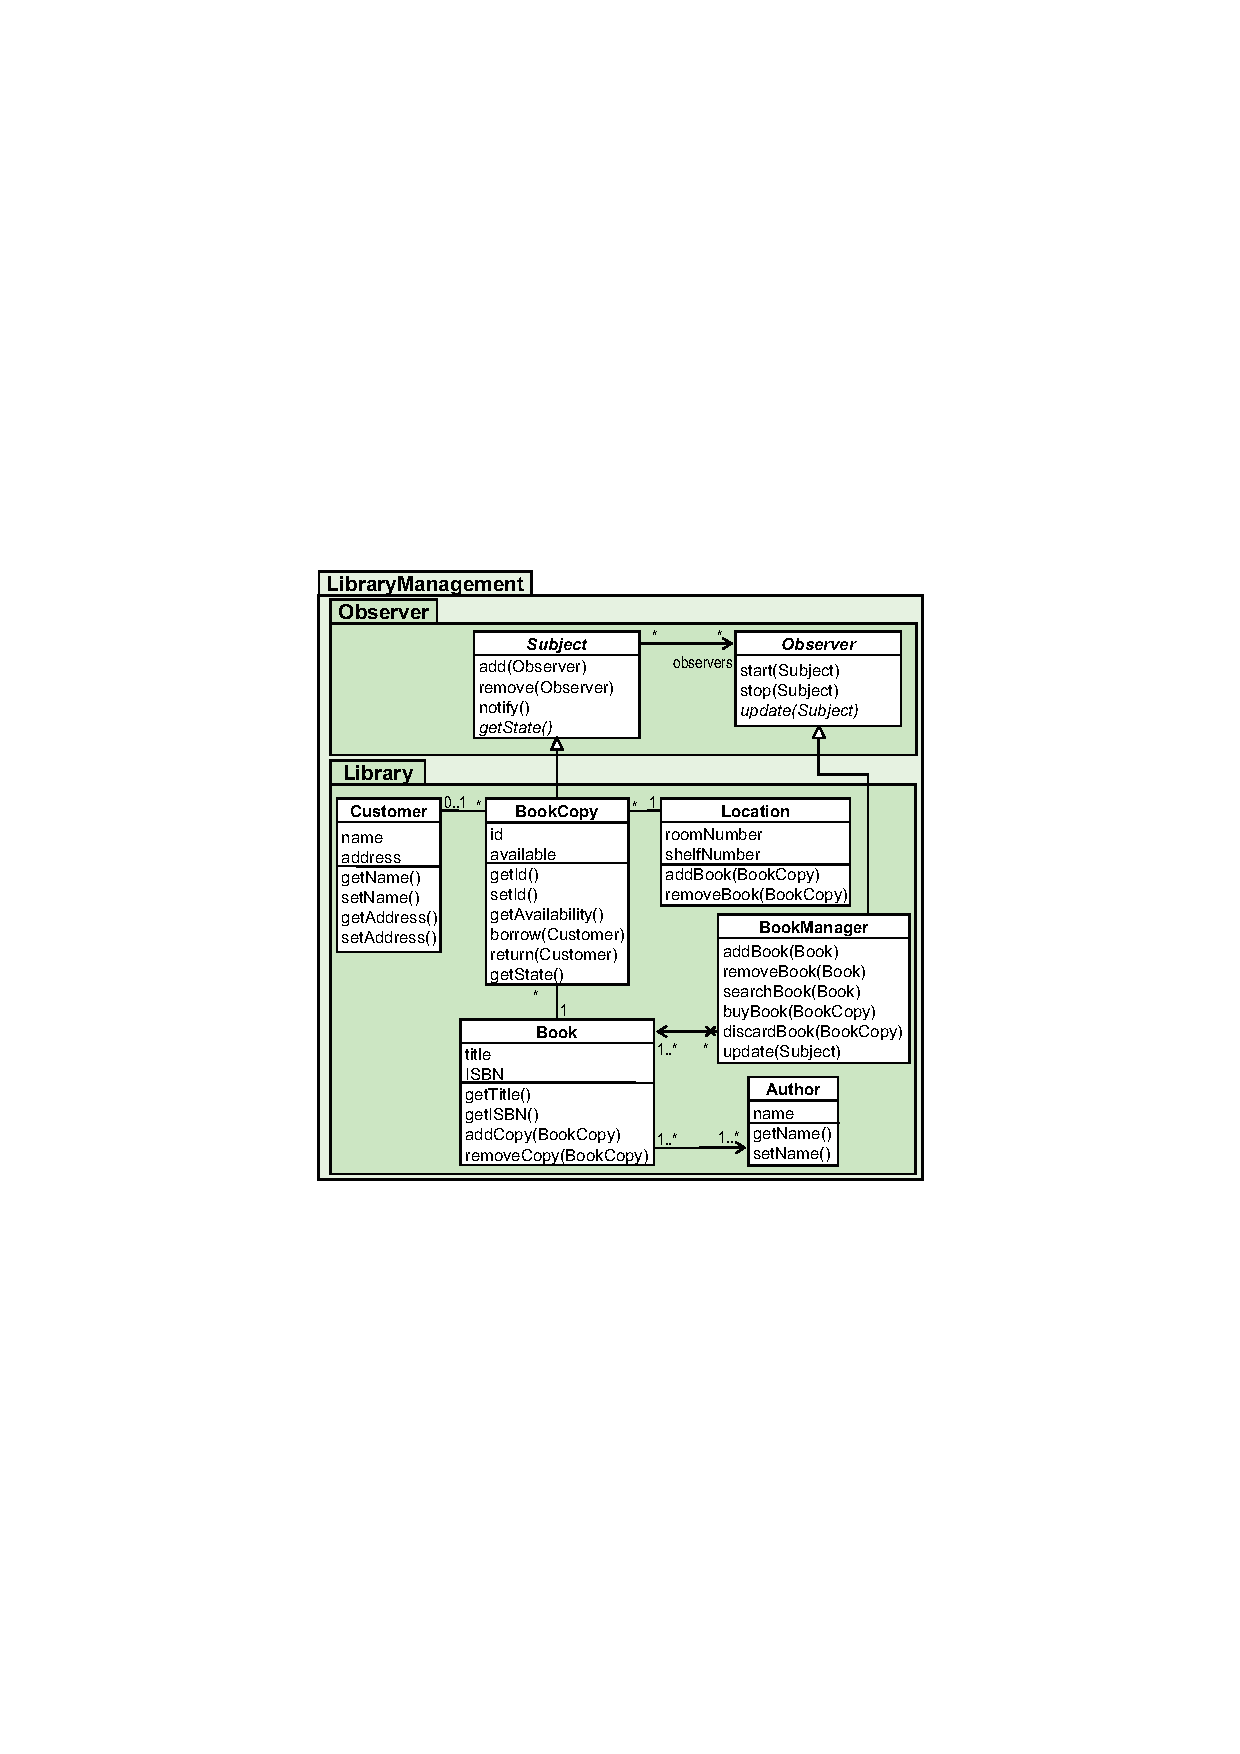
\includegraphics[width=0.4\linewidth]{figures/figure1}
	\caption{xxx (Quelle zitieren, wenn nicht selbst erstellt)}
	\label{fig:xxx}
\end{figure}

%-----------------------------------------------------------------------
\subsection{Tabellen}
%-----------------------------------------------------------------------

Jede Tabelle muss im Fließtext referenziertw werden. Für Tabellen gelten die selben Regeln, wie für Abbildungen (siehe dazu Abschnitt \ref{sec:abbildungen}).

Eine Beispiel einer Tabelle ist in Tabelle \ref{tab:xxx} zu finden:
\begin{table}
	\centering
	\begin{tabular}{| >{\bfseries}l | c | r | }
		\hline
			\rowcolor{orange} \bfseries Linksbündig & \bfseries Zentriert & \bfseries Rechtsbündig \\
		\hline
		\hline
			Zeile 1 & xxx & xxx \\\hline
			Zeile 2 & xxx & \dots \\\hline
			\multirow{2}{*}{Zeile3}
			& xxx & xxx \\\cline{2-3}
			& xxx & xxx \\\hline
		\hline
			\multicolumn{3}{| c |}{xxx} \\\hline
	\end{tabular}
	\caption{xxx (Quelle angeben)}
	\label{tab:xxx}
\end{table}

Bitte beachten Sie, dass Tabellen generell so einfach wie möglich gehalten werden sollen. Tabelle \ref{tab:xxx} dient unter anderem dazu Studierenden zu zeigen, wie Tabellen in \LaTeX\xspace erstellt werden können und wie Farben verwendet werden.